\documentclass[11pt]{article}

%\usepackage[english]{babel}
\usepackage[utf8]{vietnam}

%\usepackage[english,vietnam]{babel}
%\usepackage[utf8x]{inputenc}

%\usepackage[utf8]{inputenc}
%\usepackage[francais]{babel}
\usepackage{a4wide,amssymb,epsfig,latexsym,multicol,array,hhline,fancyhdr}
\usepackage{lastpage}

\usepackage[lined,boxed,commentsnumbered]{algorithm2e}
\usepackage{enumerate}
\usepackage{color}
\usepackage{graphicx}							% Standard graphics package
\usepackage{array}
\usepackage{tabularx}
\usepackage{multirow}
\usepackage{multicol}
\usepackage{rotating}
\usepackage{graphics}
\usepackage[a4paper,left=2cm,right=2cm,top=1.8cm,bottom=2.8cm]{geometry}
\usepackage{setspace}
\usepackage{epsfig}
\usepackage{tikz}
\usetikzlibrary{arrows,snakes,backgrounds}
\usepackage{hyperref}
\hypersetup{urlcolor=blue,linkcolor=black,citecolor=black,colorlinks=true} 
%\usepackage{pstcol} 								% PSTricks with the standard color package



%\usepackage{amsmath,amsfonts,amssymb,amsthm,epsfig,epstopdf,titling,url,array}
\usepackage{tabularx,ragged2e}
\usepackage{booktabs}
\usepackage{graphicx}
\usepackage{float}

%for long algorithm
\usepackage{algorithmicx}
%\addtolength\textheight{-32\baselineskip}
%\addtolength\paperheight{-32\baselineskip}
%\pdfpageheight\paperheight
%\renewcommand\labelenumi{\textbf{\theenumi) }}
%\usepackage[linesnumbered,algoruled,lined,boxed]{algorithm2e}
%\usepackage{algorithm}% http://ctan.org/pkg/algorithms
\usepackage{algpseudocode}% http://ctan.org/pkg/algorithmicx
\usepackage{varwidth}% http://ctan.org/pkg/varwidth

\algnewcommand\algorithmicinput{\textbf{Input:}}
\algnewcommand\INPUT{\item[\algorithmicinput]}
\algnewcommand\algorithmicoutput{\textbf{Output:}}
\algnewcommand\OUTPUT{\item[\algorithmicoutput]}


\algtext*{EndIf}% Remove "end if" text
\algtext*{EndFor}% Remove "end if" text
\algtext*{EndWhile}% Remove "end if" text

\newtheorem{theorem}{{\bf Định lý}}
\newtheorem{property}{{\bf Tính chất}}
\newtheorem{proposition}{{\bf Mệnh đề}}
\newtheorem{corollary}[proposition]{{\bf Hệ quả}}
\newtheorem{lemma}[proposition]{{\bf Bổ đề}}
\newtheorem{observation}[proposition]{{\bf Nhận xét}}

%%ensembles de nombres
\def\NP{$\mathcal{NP}$}
\def\N{\mathbb{N}}
\def\Z{\mathbb{Z}}
\def\R{\mathbb{R}}
\def\Q{\mathbb{Q}}


%\usepackage{fancyhdr}
\setlength{\headheight}{40pt}
\pagestyle{fancy}
\fancyhead{} % clear all header fields
\fancyhead[L]{
 \begin{tabular}{rl}
    \begin{picture}(25,15)(0,0)
    \put(0,-8){
\includegraphics[width=8mm, height=8mm]{hcmut.png}}
    %\put(0,-8){\epsfig{width=10mm,figure=hcmut.eps}}
   \end{picture}&
	%
\includegraphics[width=8mm, height=8mm]{hcmut.png} & %
	\begin{tabular}{l}
		\textbf{\bf \ttfamily Trường Đại Học Bách Khoa Tp.Hồ Chí Minh}\\
		\textbf{\bf \ttfamily Khoa Khoa Học và Kỹ Thuật Máy Tính}
	\end{tabular} 	
 \end{tabular}
}
\fancyhead[R]{
	\begin{tabular}{l}
		\tiny \bf \\
		\tiny \bf 
	\end{tabular}  }
\fancyfoot{} % clear all footer fields
\fancyfoot[L]{\scriptsize \ttfamily Bài tập lớn môn Giải thuật nâng cao -- Niên khóa 2020--2021}
\fancyfoot[R]{\scriptsize \ttfamily Trang {\thepage}/\pageref{LastPage}}
\renewcommand{\headrulewidth}{0.3pt}
\renewcommand{\footrulewidth}{0.3pt}


\begin{document}

\begin{titlepage}
\begin{flushleft}
\noindent Trường Đại Học Bách Khoa Tp. Hồ Chí Minh\\
Khoa Khoa Học \& Kỹ Thuật Máy Tính\\
\end{flushleft}

\vspace{1cm}

\begin{figure}[h!]
\begin{center}

\includegraphics[width=3cm]{hcmut.png}
\end{center}
\end{figure}

\vspace{1cm}


\begin{center}
\begin{tabular}{c}
\multicolumn{1}{l}{\textbf{{\Large GIẢI THUẬT NÂNG CAO}}}\\
~~\\
\hline
\\
\multicolumn{1}{l}{\textbf{{\Large Bài tập lớn}}}\\
\\
\textbf{{\Huge Xếp lại thời khóa biểu}}\\
\textbf{{\Huge cho trường học}}\\
\\
\hline
\end{tabular}
\end{center}

\vspace{3cm}

\begin{minipage}[t]{0.60\linewidth}
Tutors \\ HUYNH TUONG Nguyen
\end{minipage}
\begin{minipage}[t]{0.40\linewidth}
Student name\\
Promotion Class\\
\end{minipage}

\begin{center}
Phiên bản 1.0
\end{center}
\end{titlepage}

\newpage

\tableofcontents %summary insertion

\newpage

\title{University Course Timetabling Problem\\
Xếp lại thời khóa biểu cho trường học}
% author names and affiliations
% use a multiple column layout for up to three different
% affiliations
\author{Van Long VO, Hong Son TRANG, \\ 
Van Huy NGUYEN, Nguyen HUYNH TUONG \\
Faculty of Computer Science \& Engineering, \\ Ho Chi Minh city University of Technology, Vietnam\\
268 Lý Thường Kiệt, Hồ Chí Minh, Viet Nam\\
htnguyen@hcmut.edu.vn}
% make the title area
\maketitle



\begin{abstract}
%\boldmath
%The abstract goes here.
\noindent 
In this study, blah blah.

\end{abstract}

\small
\noindent {\bf Keywords:} transportation management; bus stop selection; bus route genenation; school bus scheduling.
 

\vspace*{1cm}


%%%%%%%%%%%%%%
\section{\texorpdfstring{Giới thiệu}{Introduction}}

$\indent$Xuất phát từ những nhu cầu phát sinh trong việc lập kế hoạch sản xuất và xây dựng các hệ thống hỗ trợ quản lý thông qua máy tính, lý thuyết lập lịch là một trong những ngành đã được đào sâu và thu hút nhiều nhà nghiên cứu trên thế giới. Ngày nay, lập lịch là một lĩnh vực quan trọng của ngành tối ưu hóa tổ hợp, và là lĩnh vực liên ngành kết hợp giữa: toán học ứng dụng, khoa học máy tính và khoa học quản lý. Theo một nghĩa rộng, lập lịch là tìm một sắp xếp các nhiệm vụ (hoặc công việc) nhằm thỏa mãn một số ràng buộc về tài nguyên hạn chế và nhằm để đáp ứng một số mục tiêu đề ra (lý thuyết lập lịch được định nghĩa và trình bày chi tiết trong nhiều sách xuất bản trên thế giới \cite{Blazewicz:al:2007, Jozefowska:2007, Leung:2004, Pinedo:2002, Tkindt:Billaut:2006}.


Lập lịch theo nghĩa rộng là một quá trình hỗ trợ quyết định cách cấp phát tài nguyên để xử lý một tập các tác vụ/công việc sao cho thỏa mãn một số ràng buộc cho sẵn. Nó đóng một vai trò quan trọng trong việc giúp đỡ con người lập kế hoạch sử dụng nguồn tài nguyên hợp lý và có hiệu quả nhất. Và do vậy, nó thường được áp dụng trong các hệ thống quản lý sản xuất công nghiệp và dịch vụ.

Khái niệm về lập lịch không phải là mới: các kim tự tháp Ai Cập đã hơn 3000 năm tuổi, Tôn Tử đã viết về việc xây dựng chiến lược quân sự 2500 năm trước đây, đường sắt xuyên lục địa đã được xây dựng trong khoảng 200 năm, … Không có bất kỳ công trình nào đã trình bày có thể được thực hiện mà không có ảnh hưởng bởi một hình thức nào đó về lập kế hoạch (hay còn gọi là lập lịch trình - sự hiểu biết các hoạt động và trình tự). Trong khi các nhà quản lý (hoặc các nhà lãnh đạo quân sự, các tổ chức chịu trách nhiệm hoàn thành công trình) phải nhận thức và đánh giá cao của lập kế hoạch (hoặc ít nhất là những người thành công cần phải có)- tuy nhiên có rất ít bằng chứng rõ ràng về một kế hoạch được xây dựng bài bản, chuẩn mực cho đến thế kỷ 20.

Từ những năm 1950, các bài toán về hỗ trợ ra quyết định đã được đào sâu và liên tục cải tiến song hành cùng với ngành khoa học quản lý tại các nước phát triển trên thế giới bởi vì nhu cầu thực tiễn của nó ngày càng tăng và do đó, các bài toán nghiên cứu học thuật ngày càng được mở rộng và sát với thực tế. Trong số những bài toán tối ưu hóa tổ hợp ứng dụng thực tiễn vào thời điểm này, đa phần thường liên quan đến bài toán lập lịch trong thế giới công nghiệp và dùng để quản lý/ tối ưu việc sử dụng các nguồn tài nguyên rất hạn chế. Và từ nền tảng cơ sở đó, các bài toán quản lý trong các lĩnh vực nghiên cứu tối ưu khác như kiến trúc máy tính \cite{Muchnick:Gibbons:2004}, viễn thông \cite{Lutton:al:2000}, giao thông vận tải \cite{Artiouchine:al:2008}, hàng không \cite{Artiouchine:al:2008, Baptiste:Sadykov:2010}, sinh tin học \cite{Blazewicz:al:2007}, tài chính \cite{Coffman:al:2010}, sức khỏe cộng đồng \cite{Kergosien:al:2011a, Kergosien:al:2011b}, … cũng đã được hưởng lợi từ những thành quả mang lại từ các bài toán lập lịch trong sản xuất.
 
%%%%%%%%%%%%%%%%%%%%%%%%%%%%%%%5
\section{\texorpdfstring{Bài toán xếp lịch}{Scheduling/Timetabling problem}}

Bài toán lập lịch là bài toán đi tìm một lập lịch thỏa mãn một số ràng buộc và mục tiêu nào đó. Các ràng buộc có thể là ràng buộc về các thuộc tính của công việc hay là ràng buộc về môi trường làm việc và khả năng của máy. Mục tiêu cần thỏa mãn ví dụ như là cực tiểu thời gian hoàn thành các công việc, công việc hoàn thành không được quá sớm cũng không quá trễ, cực tiểu thời gian trễ so với thời gian hoàn thành dự kiến $\ldots$ hoặc là sự kết hợp của nhiều mục tiêu khác nhau.
Một số khái niệm liên quan về lập lịch: 

\begin{itemize}
\item Một lập lịch khả dĩ: là một lập lịch sao cho: 
  \begin{itemize}
    \item Không có 2 khoảng thời gian nào trùng lặp nhau trên cùng một máy.
    \item Không có 2 khoảng thời gian nào trùng lắp được cấp phát cho cùng 1 công việc .
    \item Thỏa mãn một số đặc điểm của vấn đề đặc trưng. 
  \end{itemize}
\item Một lập lịch tối ưu là một lập lịch cực tiểu một mục tiêu tối ưu mong muốn. 
\end{itemize}
 
Trong ngữ cảnh lập lịch trong trường học, bài toán xếp thời khóa biểu là bài toán nhận được rất nhiều sự quan tâm bởi các nhà nghiên cứu trên thế giới. Đây là một dạng bài toán lập lịch mà có hạn chế về nguồn lực liên quan đến việc phân bổ một nhóm các khóa học vào một nhóm khung thời gian, theo cách thức để tối ưu hóa một tập hợp các mục tiêu mong muốn. Hai bài toán kinh điển nổi tiếng trong lĩnh vực này là bài toán giáo viên đứng lớp và bài toán xếp thời gian khóa học đại học (UCTP - University Course Timetabling Problem).

Mô hình lớp học - giáo viên, được giới thiệu bởi Gotlieb (1963) \cite{Gotlieb:1963}, trong đó một tập hợp các giảng viên nên được chỉ định cho một nhóm lớp học và khoảng thời gian nhất định. Trong bài toán đề cập, có nhiều lớp học mà mỗi một lớp học bao gồm một nhóm học sinh theo cùng một chương trình. Giả sử rằng tất cả các bài giảng đều có thời lượng như nhau, Asratian và de Werra (2002) \cite{Asratian:deWerra:2002} đã xem xét một bài toán xếp thời biểu tương ứng với một số tình huống thường xuyên xảy ra trong chương trình đào tạo cơ bản của các trường đại học và phổ thông. Thời gian biểu của trường đại học bao gồm thời gian biểu của kỳ thi cũng như thời gian biểu của khóa học. Xếp bảng biểu lịch kiểm tra lần đầu tiên được công bố bởi Carter, Laporte và Lee (1996) \cite{Carter:al:1996} và được định nghĩa là: “Việc chỉ định các kỳ kiểm tra trong một số khoảng thời gian có sẵn theo cách mà không có xung đột hoặc đụng độ.” Như một mô tả ngắn gọn, bài toán này là phân bổ một tập hợp các bài kiểm tra vào một tập khung thời gian nhất định để không có học sinh nào được sắp xếp thời gian cho hai kỳ thi khác nhau tại một lúc.
 
%%%%%%%%%%%%%%%%%%%%%%
\section{\texorpdfstring{Các phương pháp tiếp cận}{Approaches}}

Nhờ vào sự tiến bộ và hỗ trợ của máy tính, các bài toán và thuật toán trong lập lịch ngày càng đa dạng, gần gũi với thực tế, và thực sự thu hút các nhà nghiên cứu quan tâm đến giải quyết những bài toán có tính thách thức cao.
Dựa theo các thuật toán và các phương pháp tiếp cận, chúng có thể được phân nhỏ thành một số loại như sau:

\begin{itemize}
\item Đo độ khó của bài toán: Brucker \cite{Brucker:2004,Brucker:Knust:2004} xây dựng một bảng tổng kết độ khó của các bài toán lập lịch đã được nghiên cứu; ngoài ra một vài công trình nổi bật khác cũng có thể tham khảo thêm, như là các công trình của Timkovsky về việc so sánh độ khó giữa các nhóm bài toán lập lịch \cite{Timkovsky:1998,Timkovsky:2003}, hoặc có thể tham khảo bài toán lập lịch đầu tiên được chứng minh bởi Johnson \cite{Johnson:1954}, hoặc một vài kết quả khác \cite{Haned:al:2012, Soukhal:al:2005}.

\item Xác định cận biên $P \neq NP$(maximal polynomial solvable): một số nghiên cứu quan tâm đến cận giới hạn trong các bài toán lập lịch  \cite{Baptiste:2000, Baptiste:al:2004, Baptiste:al:2007, Brucker:2004, HuynhTuong:Soukhal:2008}.

\item Phương pháp tính chính xác: quy hoạch nguyên \cite{Baptiste:Sadykov:2010, LeThi:Pham:2008}, quy hoạch động \cite{HuynhTuong:al:2010, Lawler:1969, Lawler:1990}, phương pháp tính cận và nhánh \cite{BellenguezMorineau:Neron:2007, Carlier:1982, Woeginger:2008}.

\item Các giải thuật gần đúng dựa trên phương pháp tính chính xác: thuật giải gần đúng cho quy hoạch phi tuyến tính (linear programming)\cite{Hoang:2009a, Hoang:2009b, LeThi:Pham:2008}; xây dựng chuỗi giải thuật gần đúng có đảm bảo chắc chắn được chất lượng của giải pháp tìm thấy (approximation scheme \cite{Afrati:Milis:2006, Kellerer:Strusevich:2006, Kolliopoulos:Steiner:2006, Kovalyov:1995}); thuật giải gần đúng dựa trên cây quyết định (branch and cut, branch and price, search tree based approaches \cite{Neron:al:2008, Woeginger:2008}, recovering beam search \cite{DellaCroce:al:2011, Rakrouki:al:2012}, relaxation, hiệu chỉnh cấu hình của solver giải hiệu quả các bài toán quy hoạch tuyến tính, . . . 

\item Các thuật toán tiến hóa: thuật giải di truyền \cite{Holland:1975, Soukhal:al:2005}, tìm kiếm lân cận, meta-heuristic \cite{Kergosien:al:2011a}, thuật giải lai (hybrid) \cite{Rakrouki:al:2012}, $\ldots$
\end{itemize}


%%%%%%%%%%%%%%%%%%%%%%%%%
\section{\texorpdfstring{Các công trình nghiên cứu liên quan về xếp thời biểu trong nhà trường}{Related works of UCTP}}

UCTP được Carter và Laporte (1997) \cite{Carter:Laporte:1997} mô tả như sau: “Một bài toán phân công đa chiều, trong đó sinh viên, giáo viên (hoặc giảng viên) được chỉ định cho các khóa học, một phần khóa học hoặc lớp học; "các sự kiện" (các cuộc họp cá nhân giữa học sinh và giáo viên) được gán vào các lớp học và các khung thời gian. " Gần giống với các vấn đề tính toán thời gian khác, bài toán này, là NP-hard, bao gồm cả các ràng buộc mềm và cứng. Liên quan đến những hạn chế cứng, một số trong số những ràng buộc được áp dụng trong tài liệu được liệt kê dưới đây.

\begin{enumerate}[I.]
\item Đối với mỗi khung thời gian trong mỗi phòng, chỉ một nhóm sinh viên và một giáo sư có thể tham dự.

\item Không cho phép nhiều hơn một khóa học cho mỗi khung thời gian trong mỗi phòng.

\item Số lượng học viên tham gia khóa học phải nhỏ hơn hoặc bằng sức chứa của phòng.

\item Căn phòng phải đáp ứng các chức năng theo yêu cầu của khóa học (tham khảo Cacchiani, Caprara, Roberti, \& Toth, 2013 \cite{Cacchiani:al:2013}; Lewis, Paechter, \& McCollum, 2007 \cite{Lewis:al:2007}).

\item Khi được chỉ định, một khóa học phải được lên lịch trong khung thời gian được xác định trước (tham khảo Goh, Kendall, \& Sabar, 2017 \cite{Goh:al:2017}; Lewis \& Thompson, 2015 \cite{Lewis:Thompson:2015}).

\item Để đáp ứng các yêu cầu về ưu tiên, các khóa học phải được lên lịch diễn ra theo đúng thứ tự (tham khảo Babaei, Karimpour, \& Hadidi, 2015 \cite{Babaei:al:2015}).
\end{enumerate}

Ngoài ra, có rất nhiều ràng buộc mềm được sử dụng trong các bài toán khác nhau, trong đó một số ràng buộc được đưa ra như sau.

\begin{enumerate}[I.]
\item Các khóa học nên được sắp xếp theo cách giảm thiểu khung thời gian trống của cả giáo sư và sinh viên (tham khảo Lewis \& Thompson \cite{Lewis:Thompson:2015}; Van den Broek \& Hurkens, 2012 \cite{VandenBroek:Hurkens:2012}).

\item Sinh viên không nên chỉ tham gia một khóa học trong một ngày (tham khảo Goh và cộng sự, 2017; Lewis \& Thompson, 2015 \cite{Lewis:Thompson:2015}).

\item Các khóa học không nên được lên lịch vào khoảng thời gian cuối cùng của một ngày (tham khảo Henry Obit, 2010 \cite{HenryObit:2010}).

\item Tốt hơn là một khóa học được giảng dạy trong một phòng cụ thể do giáo sư yêu cầu (tham khảo công trình của Lewis và cộng sự công bố năm 2007 \cite{Lewis:al:2007}).

\item Vào mỗi ngày, một khoảng thời gian nên được bỏ trống để học sinh nghỉ trưa (tham khảo Lewis và cộng sự  \cite{Lewis:al:2007}).
\end{enumerate}

Cacchiani và cộng sự. (2013) \cite{Cacchiani:al:2013} đã giải quyết các UCTP bằng hai cách tiếp cận chung: Xếp thời gian biểu khóa học dựa trên Chương trình giảng dạy (Curriculum-based UTCP) và xếp thời gian biểu khóa học dựa trên sự đăng ký của từng sinh viên (Post Enrollment-based UTCP).

Về cách tiếp cận đầu tiên, sinh viên được phân loại thành “nhóm” dựa trên chương trình học và các khóa học cần thiết để đáp ứng nhu cầu chương trình học cho học kỳ tiếp theo của họ; nói cách khác, mỗi nhóm tính đến chương trình giảng dạy cũng như các khóa học phải tuân theo và thực hiện mỗi học kỳ (tham khảo Cacchiani và cộng sự, 2013 \cite{Cacchiani:al:2013}). Vấn đề sau đó là tạo ra các lịch bài giảng mà xung đột giữa các khóa học được thiết lập cho phù hợp với chương trình giảng dạy được chỉ định.

Trong cách tiếp cận thứ hai, Bảng thời gian khóa học dựa trên sự đăng ký, việc lên lịch được xác định dựa trên dữ liệu ghi danh của từng học sinh riêng lẻ, sao cho tất cả học sinh có thể tham gia các khóa học mà họ đã đăng ký. Có một số nghiên cứu gần đây trong lĩnh vực này như Abdullah và Turabieh (2012) \cite{Abdullah:Turabieh:2012}, Cambazard, Hebrard, O'Sullivan, và Papadopoulos (2012) \cite{Cambazard:al:2012}, Ceschia, Di Gaspero, và Schaerf (2012) \cite{Ceschia:al:2012}, Méndez-Díaz, Zabala, và Miranda-Bront (2016) \cite{Mendez-Diaz:al:2016}. Lewis và cộng sự. (2007) \cite{Lewis:al:2007} đã đưa ra mô tả về loại vấn đề này được sử dụng cho Track Two của Second International Timetabling Competition.

Tổng quan các phương pháp/giải pháp tiếp cận, các kỹ thuật áp dụng để giải quyết UCTP được trình bày bởi Babaei et al. (2015) \cite{Babaei:al:2015} như sau:

\begin{enumerate}[a.]
\item Vận trù học (OR),
\item Phương pháp siêu mô phỏng,
\item đa tiêu chí và kỹ thuật đa mục tiêu,
\item phương pháp tiếp cận mới liên quan đến trí tuệ nhân tạo
\item và cách tiếp cận hệ thống đa đại lý phân tán.
\end{enumerate}

Phương pháp tô màu đồ thị (graph coloring method), một trong những kỹ thuật dựa trên vận trù học (OR), lần đầu tiên được đề cập bởi Welsh và Powell (1967) \cite{Welsh:Powell:1967}, tuy nhiên, phương pháp này không giải quyết được các trường hợp với các khóa học được chỉ định trước. Sử dụng một cách tiếp cận gần như tương tự, De Werra (1985) \cite{DeWerra:1985} đã đề xuất một công thức cho bài toán về tô màu cạnh trong đa đồ thị lưỡng phân trong đó các nút là các lớp và các giáo viên, các ràng buộc được xác định bởi các cạnh và mỗi khoảng thời gian tương ứng với một màu sắc. Để phát triển một cách tiếp cận hiệu quả hơn về thời gian chạy và hiệu suất thể dục, Asham, Soliman và Ramadan (2011) \cite{Asham:al:2011} đã sử dụng màu biểu đồ và thuật toán di truyền (GA - Genetic Algorithm) như một giải pháp kết hợp.

Theo tài liệu, quy hoạch tuyến tính là một tập hợp con trong vận trù học, được sử dụng rộng rãi trong các bài toán xếp lịch. Mô hình được phát triển bởi Bakir và Aksop (2008) \cite{Bakir:Aksop:2008} dựa trên cách tiếp cận đã đề cập, trong đó thời gian biểu sắp xếp khóa học tối ưu đạt được bằng cách sử dụng mô hình quy hoạch nguyên 0-1, trong đó sự không hài lòng cả sinh viên và giảng viên được giảm thiểu và tập các ràng buộc được hiện thực để áp dụng các quy tắc.

Khi cần xem xét kỹ hơn các tài liệu liên quan, chúng ta cũng nên tham khảo Lewis (2008) \cite{Lewis:2008} là một trong số nhà nghiên cứu đã phân loại các thuật toán siêu mô phỏng để xếp lịch thời biểu thành ba nhóm: (a) Thuật toán tối ưu hóa một giai đoạn, (b) Thuật toán tối ưu hóa hai giai đoạn và ( c) Các thuật toán cho phép thư giãn.

Alvarez-Valdes, Crespo, và Tamarit (2002) \cite{Alvarez-Valdes:al:2002} đã sử dụng tìm kiếm tabu (TS - Tabu Search) để giải quyết bài toán UTCP trong ba giai đoạn và xây dựng một thời khóa biểu phù hợp với đặc điểm của hệ thống đại học Tây Ban Nha . Phương pháp giải này cũng đã được Goh et al. (2017) \cite{Goh:al:2017}, nơi nó được kết hợp với ủ mô phỏng (SA – Simulated Annealing) để cải thiện chất lượng giải pháp của các giải pháp khả thi. 

Việc tối ưu hóa tổ hợp cũng được giải quyết bởi Tuga, Berretta và Mendes (2007) \cite{Tuga:al:2007}, trong đó các tác giả cung cấp sự kết hợp của chuỗi lân cận Kempe trong thuật toán SA. Trong cách tiếp cận của họ, một giải pháp khả thi được tạo ra dựa trên đồ thị dựa trên heuristic và thuật toán SA, được sử dụng để giảm thiểu vi phạm các ràng buộc mềm. 

Khonggamnerd và Innet (2009) \cite{Khonggamnerd:Innet:2009} nghiên cứu một phương pháp tổng hợp khác để giải quyết vấn đề sắp xếp thời khóa biểu của trường đại học, trong đó mô hình thuật toán di truyền được áp dụng để cải thiện hiệu quả của việc sắp xếp tự động thời khóa biểu của trường đại học. 

Song, Liu, Tang, Peng và Chen (2018) \cite{Song:al:2018} tập trung vào thuật toán tìm kiếm cục bộ lặp đi lặp lại để tìm ra giải pháp khả thi cho UCTP. Kết quả tính toán trong bài báo này cho thấy thuật toán được phát triển của họ đạt được kết quả cạnh tranh cao so với các thuật toán hiện có.

Phương pháp luận mờ, được coi là trong nhóm các phương pháp tiếp cận mới liên quan đến trí tuệ nhân tạo, lần đầu tiên được giới thiệu bởi Zadeh (1965) \cite{Zadeh:1965} và đã được sử dụng rộng rãi trong một loạt các ứng dụng trong thế giới thực. Trong UCTP, Chaudhuri và De (2010) \cite{Chaudhuri:De:2010} đã phát triển một thuật toán di truyền mờ để các mô hình tập mờ đo lường sự vi phạm các ràng buộc mềm trong hàm phù hợp để kiểm soát sự không chắc chắn và mơ hồ vốn có liên quan đến dữ liệu cuộc sống thực.

Tuy nhiên, trong các tình huống thực tế, có một sự không chắc chắn cố hữu về tổng số sinh viên sẽ đăng ký cho mỗi khóa học. Vì trạng thái cuối cùng của mỗi khóa học, cho dù nó được giữ trong thời khóa biểu hay bị hủy bỏ, được xác định dựa trên dữ liệu đăng ký của tất cả học sinh, nên việc xử lý sự không rõ ràng về vấn đề này chắc chắn sẽ rất hiệu quả. 

Chúng ta đều biết rằng các mô hình thời gian biểu sau khi đăng ký khóa học là để giải quyết vấn đề này bằng cách lên lịch dựa trên các lựa chọn của sinh viên, không phải chương trình giảng dạy của trường đại học. Tuy nhiên, ở một số trường đại học, khoảng thời gian từ khi sinh viên đăng ký đến học kỳ tiếp theo là ngắn và điểm vẫn không được công bố trong kỳ nhập học. Do đó, có thể có một sự thay đổi đáng kể trong danh sách tổng kết  các học sinh sau thời gian hủy bỏ hoặc đăng ký bổ sung. Điều đáng nói là tầm quan trọng của việc đối phó với sự không chắc chắn này được nêu bật khi tính đến sự hài lòng chung của sinh viên và giáo sư. Giảm thiểu khoảng cách thời gian, hay còn gọi là thời gian nhàn rỗi giữa hai tiết học của một sinh viên hoặc một giáo sư, nên được coi là một hạn chế mềm trong vấn đề này, vốn chưa xuất hiện trong tài liệu. Nói cách khác, sinh viên và giáo sư mong muốn có một thời gian biểu gọn gàng và không bị chênh lệch thời gian giữa hai khóa học được lên lịch trong một ngày nhất định.



%%%%%%%%%%%%%%
\section{\texorpdfstring{Hiện trạng}{Context}}


Chương trình học tại trường Cao Đẳng Công Nghệ Quốc Tế Lilama 2 (Lilama 2 International Technology College) bao gồm hai hệ đào tạo theo niên khóa: chương trình trung cấp và chương trình đào tạo bậc cao đẳng. 
Chương trình trung cấp có chỉ tiêu tuyển sinh hàng năm khoảng 500 và có hai dạng đào tạo: 

\begin{itemize}
\item	Học viên học trong hai năm nếu đã có bằng tốt nghiệp phổ thông trung học, nghĩa là học viên cần phải hoàn thành các môn học trong chương trình đào tạo trong vòng 4 học kỳ.
\item	Học viên tốt nghiệp trung học cơ sở và có định hướng nghề nghiệp rõ ràng. Với nhóm đối tượng này, chương trình học sẽ kéo dài 3 năm, đi song hành với kiến thức văn hóa cần thu thập ở cấp trung học phổ thông. Trong mỗi ngày học, người học viên sẽ tham gia một buổi học văn hóa và một buổi theo chương trình hướng nghiệp. Sau ba năm, học viên vẫn phải thi tốt nghiệp phổ thông quốc gia và đồng thời thi tốt nghiệp trung cấp nghề, nghĩa là học viên sau ba năm học sẽ có hai bằng cấp.
\end{itemize}

Chương trình Cao đẳng có chỉ tiêu tuyển sinh hàng năm khoảng 600 và có hai dạng đào tạo:

\begin{itemize}
\item	Chương trình đào tạo cao đẳng trong nước, theo chương trình khung đào tạo do tổng cục giáo dục nghề nghiệp ban hành. Học viên học trong ba năm, nghĩa là học viên cần phải hoàn thành các môn học trong chương trình đào tạo trong vòng 6 học kỳ.
\item	Chương trình đào tạo cao đẳng nâng cao quốc tế, theo chương  trình của hiệp hội đào tạo nghề vương quốc Anh City \& Guild. Học viên học trong 3 năm rưỡi, nghĩa là học viên cần phải hoàn thành các môn học trong chương trình đào tạo trong vòng 7 học kỳ. Chương trình này kéo dài hơn hệ cao đẳng trong nước một học kỳ nhằm mục đích để đào tạo thêm về trình độ ngoại ngữ giao tiếp chuyên môn.
\end{itemize}

Mỗi lớp học tối đa gồm 35 học viên theo quy định của Tổng cục Giáo Dục Nghề Nghiệp. Tổng cộng trung bình hàng năm, nhà trường cần lên kế hoạch đào tạo cho khoảng 96 lớp. Trong mỗi học kỳ, một lớp học cần học tối thiểu là 7 môn và sẽ có tiến độ học khác nhau. Nhìn chung, nhà trường cần xếp lịch cho 672 môn học trong một học kỳ.

Điểm đặc thù trong các chương trình đào tạo hướng nghiệp là đào tạo theo dạng mô đun, nghĩa là một môn học chuyên ngành sẽ có thể có nhiều mô đun. Ví dụ, môn học “Chế tạo nhà thép tiền chế” trong chương trình đào tạo cao đẳng sẽ có 3 mô đun: thiết kế bản vẽ, gia công vật tư, thi công nhà thép.

Và để thống nhất trong việc trình bày, người viết xem các môn học chung chỉ gồm một mô đun (ví dụ như là môn triết học, pháp luật, $\ldots$ ). Và giả định rằng, một mô đun là đơn vị cơ bản cần xếp thời khóa biểu và mỗi mô đun cần hoàn tất đào tạo trong một học kỳ.

Giả định rằng:
\begin{itemize}
\item	Phòng học là không giới hạn. Vì trên thực tế:
\begin{itemize}
	\item Các phòng dạy lý thuyết thì rộng và khá nhiều. 
	\item Phòng thực hành cần được quản lý bởi các giảng viên hướng dẫn chuyên môn. Hầu như mỗi giảng viên chuyên môn ngoài việc giảng dạy, đều có phụ cấp trách nhiệm và phải phụ trách đảm bảo việc vận hành của các phòng thí nghiệm. Và do đó, việc gán lịch các giảng viên chuyên môn cũng đồng thời liên quan đến việc cấp phát phòng.
\end{itemize}
\item	Giảng viên chuyên môn không giới hạn 
\item	Mỗi mô đun có thể có nhiều giảng viên tham gia giảng dạy với nhiều buổi khác nhau
\end{itemize}

Như vậy, một lịch biểu khả thi cần phải thỏa mãn các ràng buộc sau:
\begin{itemize}
\item	Không thể cho phép một lớp học nhiều mô đun trong cùng một buổihọc 
\item	Không thể cho phép một lớp được nhiều giáo viên dạy trong cùng một buổi học
\item	Không thể cho phép một giáo viên dạy nhiều mô đun khác nhau trong cùng một buổi.
\item	Với mỗi mô đun thuộc nhóm NM2, không thể cho phép một giáo viên dạy nhiều lớp cùng một buổi.
\item	Số buổi dạy của một mô đun phải đáp ứng đủ khối lượng giảng dạy yêu cầu. 
\end{itemize}

Ghi chú:
-	Khi đổi lịch để chèn một số buổi của lớp vừa thực tập xong, cần phải đảm bảo việc không làm trễ và mất buổi dạy của các lớp khác.

%%%%%%%%%%5
\subsection{\texorpdfstring{Quy trình xếp thời khóa biểu hiện tại của trường}{Current process}}
Bắt đầu năm học phòng Đào tạo sẽ lên kế hoạch đào tạo tổng thể cho toàn trường

\begin{figure}[h!]
\begin{center}
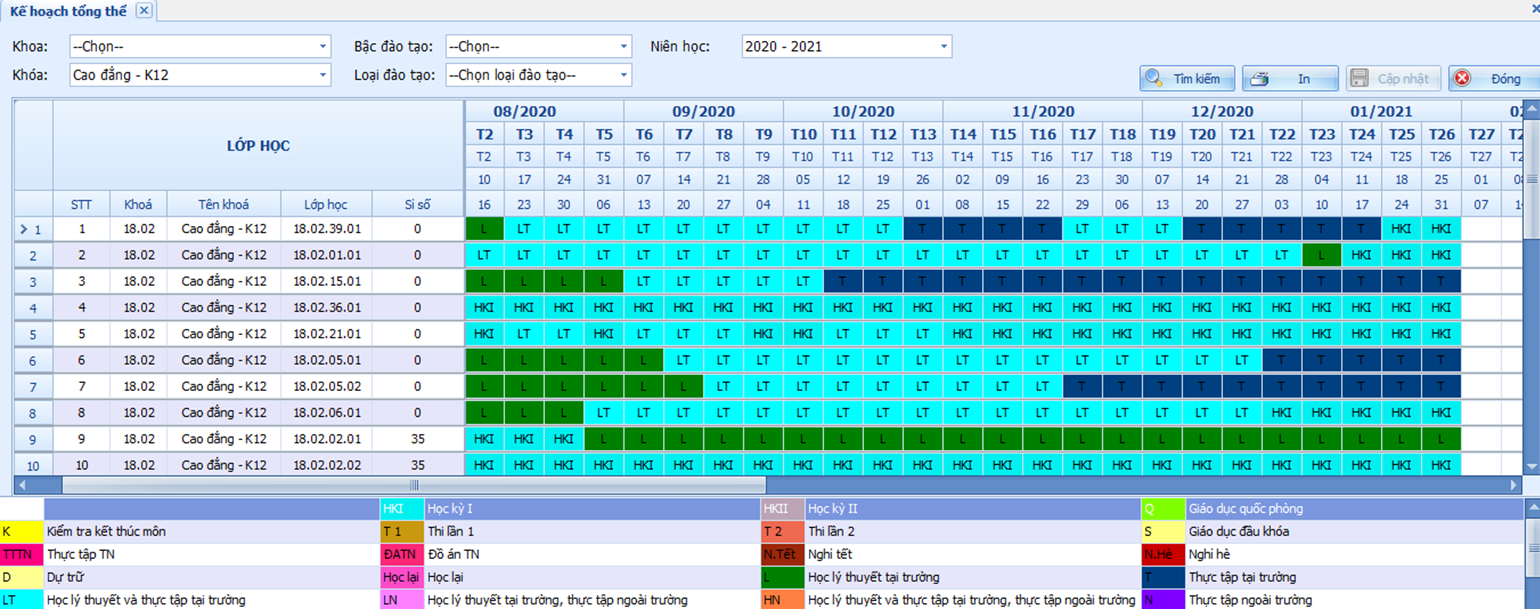
\includegraphics[width=17cm]{CurrentProcess1.png}
\caption{Thời khóa biểu}
\end{center}
\end{figure}

Ở form này phòng Đào tạo sẽ quy định thời gian bắt đầu và kết thúc học kỳ, thời gian nghỉ lễ, tết…

Tiếp theo các khoa sẽ lên danh sách môn học trong học kỳ cho lớp học:
\begin{figure}[h!]
\begin{center}
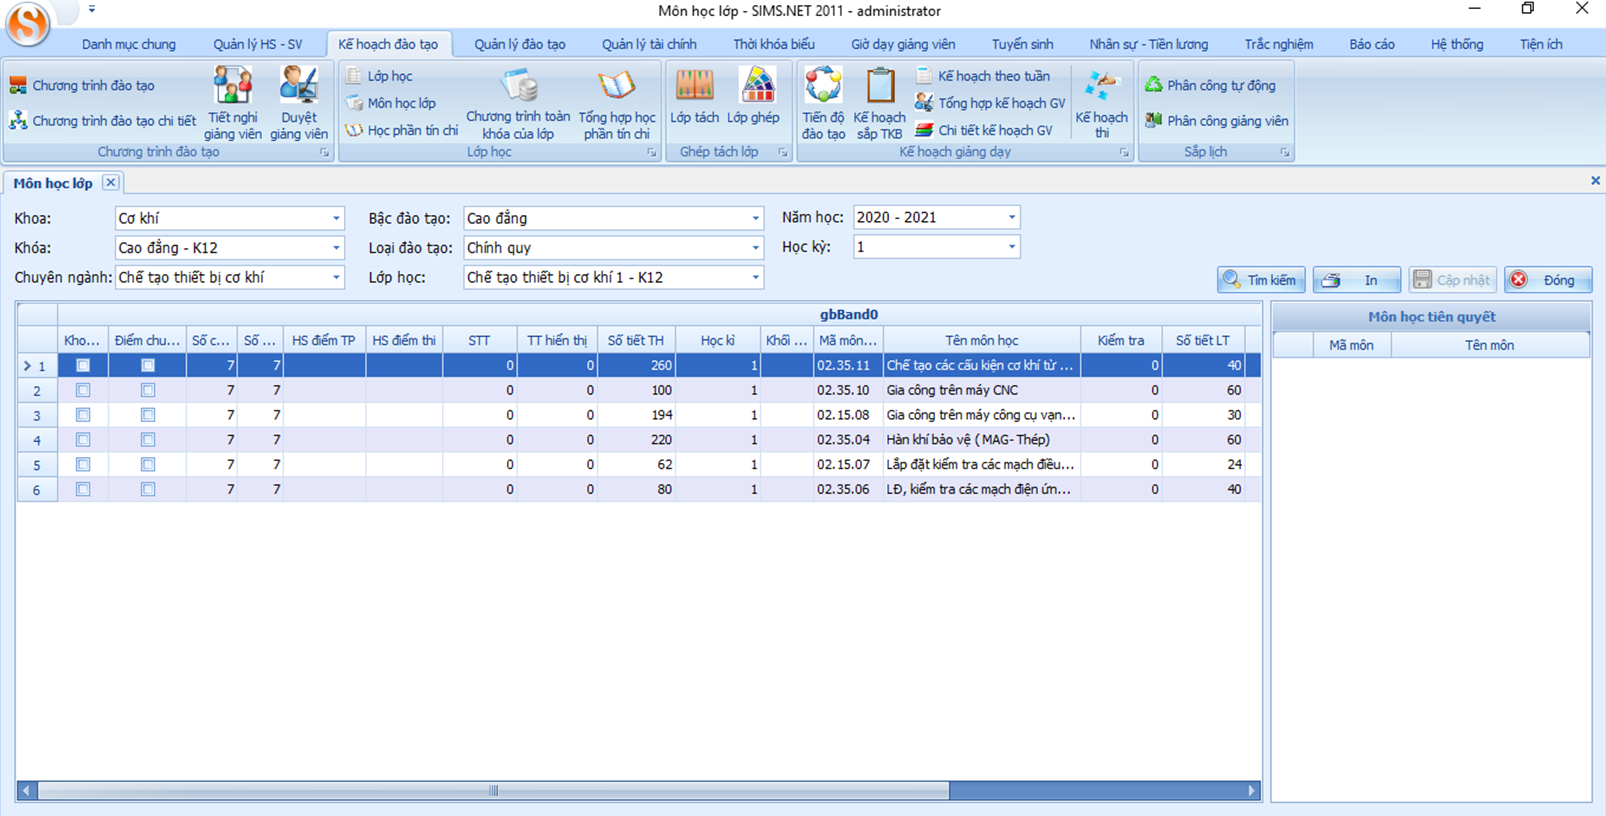
\includegraphics[width=17cm]{CurrentProcess2.png}
\caption{Môn học lớp}
\end{center}
\end{figure}

Trong form này, chọn lớp học, chọn năm học và học kỳ để thêm môn học vào cho lớp này (Ở hình 3.1) lớp Chế tạo thiết bị cơ khí 1, trong học kỳ 1 năm 2020 được bố trí 6 môn học.

Tiếp theo lên kế hoạch đào tạo và kế hoạch giảng viên  cho từng môn học trong lớp:

\begin{figure}[h!]
\begin{center}
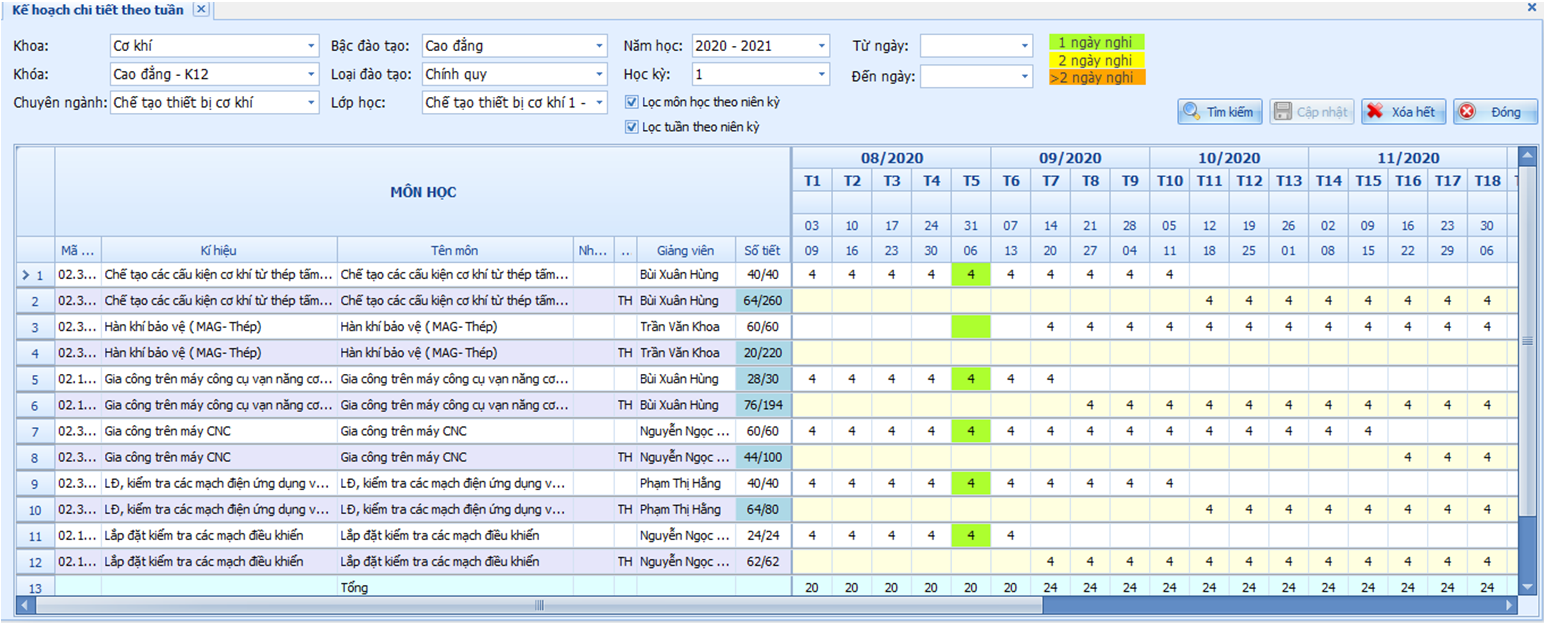
\includegraphics[width=17cm]{CurrentProcess3.png}
\caption{Kế hoạch đào tạo chi tiết theo tuần}
\end{center}
\end{figure}

Trong Form này sẽ lên kế hoạch thời gian đào tạo của từng môn theo tuần (1 buổi/tuần sẽ là 4 (tiết) và 2 buổi/tuần sẽ là 8 (tiết). , và quy định giáo viên phụ trách môn học.

Sau khi có kế hoạch giảng viên phụ trách môn học và thời lượng học của từng môn/tuần thì tiến hành sắp thời khóa biểu.

\begin{figure}[h!]
\begin{center}
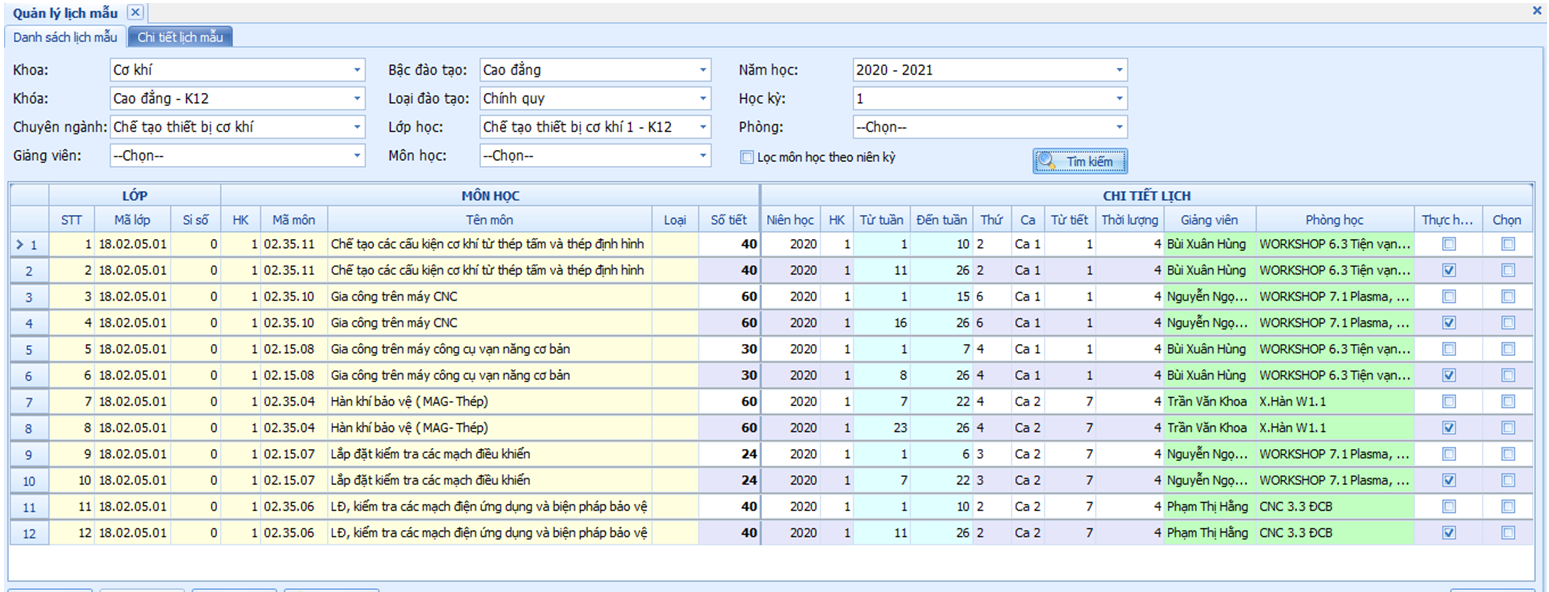
\includegraphics[width=17cm]{CurrentProcess4.png}
\caption{Gán giảng viên}
\end{center}
\end{figure}


Quá trình đi thực tập sản xuất:

\begin{itemize}
\item	Bắt đầu từ năm học thứ 2, sinh viên học các môn học chuyên môn nghề kết hợp đi thực tập sản xuất tại các công ty gắn kết với nhà trường. Kế hoạch đi  thực tập thường không có kế hoạch trước, khi doanh nghiệp bố trí được để tiếp nhận sinh viên sẽ thông báo đến nhà trường. 
\item	Nhà trường sẽ giao khoa làm quyết định đi thực tập, quyết định được chuyển về phòng đào tạo để theo dõi tiến độ.
\end{itemize}

Sau khi sinh viên kết thúc lịch thực tập sản xuất tại công ty các khoa sẽ sắp xếp lịch học cho sinh viên. Lịch học sẽ ưu tiên sử dụng lịch của đầu kỳ, ngoài ra còn tăng thêm buổi học để cho kịp tiến độ trong học kỳ



%%%%%%%%%%%%%%
\subsection{\texorpdfstring{Mô tả bài toán}{Problem statement}}


Bài toán cốt lõi ở đây không phải là “\textit{xác định một lời giải khả thi để các lớp có thể hoàn thành đúng tiến độ}”, mà là “\textit{cần sắp lịch chèn có một số lớp vào thời khóa biểu đã dự kiến trước}” do các lớp này có sự cố tạm ngừng việc học ngoài dự kiến để tham gia thực tập tại các doanh nghiệp.

Mục tiêu chính của bài toán là “\textit{xác định một lời giải mới để có thể chèn vài mô đun vào và không ảnh hướng nhiều đến các lớp đã được sắp lịch và làm sao để chương trình học hoàn thành đúng tiến độ cho nhiều lớp nhất có thể}”.

Hay nói cách khác một cách chi tiết hơn, với một thời khóa biểu của toàn trường đã cho trước (bao gồm lịch học của môn học lớp kèm với giảng viên), cần tìm lịch bổ sung sao cho có thể thêm nhiều nhất có thể số lượng môn học lớp dựa trên một danh sách (môn học lớp, giảng viên, số lượng buổi, độ ưu tiên).

%%%%%%%%%%%%%%
\subsection{\texorpdfstring{Hàm mục tiêu cần tối ưu của bài toán}{Objective function}}

Cần xử lý giải quyết tốt các sự kiện, có nghĩa là phải bổ sung vào lịch đã có sẵn. hay nói cách khác, cần xác định lịch để có thể thêm tối đa số buổi bù trong khung thời gian cho trước.

%%%%%%%%%%%%%%
\section{\texorpdfstring{Giải pháp đề xuất}{Proposed approach}}

\subsection{\texorpdfstring{Mô hình hóa toán học}{Modeling}}

Đặt $e_{(i,j,k,t)}$ là thông số mô tả thông tin lớp $L_i$ có được học môn Mj giảng viên $G_k$ tại buổi $B_t$ hay không. 
Nghĩa là khi $e_{(i,j,k,t)} = 1$, $L_i$ có được học mô đun $M_j$ giảng viên $G_k$ tại buổi $B_t$; 
và ngược lại thì $e_{(i,j,k,t)} = 0$. 
Lưu ý rằng: bộ thông số $e_{(i,j,k,t)}$ cần phải thỏa mãn ràng buộc trình bày ở mục trên.

Gọi $n_{(i,j)}$ là số buổi cần học của mô đun $j$ cho lớp thứ $i$.

Gọi $c_{(j,k)} \in \{0,1\}$ mô tả khả năng giảng dạy mô đun $j$ của giảng viên $k$. 
Nghĩa là $c_{(j,k)} = 1$ nếu và chỉ nếu giảng viên $k$ dạy được mô đun $j$ ngoài ra $c_{(j,k)} = 0$.

Điều cần làm là bổ sung thông tin của lớp $L_{i_0}$ học môn $M_{j_0}$ bởi giảng viên $G_{k_0}$  trong $n_{t_0}$ buổi.

Quyết định cho thời khóa biểu mới sẽ được mô tả bởi biến: $x_{(i,j,k,t)} \in \{0,1\}$. 

Nghĩa là nếu $x_{(i_0,j_0,k_0, t)} = 1$, $L_{i_0}$ có được học môn $M_{j_0}$ giảng viên $G_{k_0}$ tại buổi $B_t$; 
và ngược lại thì $x_{(i_0,j_0,k_0, t)} = 0$.

Bộ tập hợp biến ra quyết định $x_{(i,j,k,t)}$ cần phải thỏa mãn ràng buộc trình bày ở mục trên, chi tiết như sau:
\begin{itemize}
\item	Giảng viên $k$ không thể dạy mô đun $j$ nếu không có chuyên môn phù hợp

\item	Không thể cho phép một lớp học nhiều mô đun trong cùng một buổihọc và không thể cho phép một lớp được nhiều giáo viên dạy trong cùng một buổihọc:

\item	Không thể cho phép một giáo viên dạy nhiều mô đun khác nhau trong cùng một buổi.

\item	Với mỗi mô đun thuộc nhóm NM2, không thể cho phép một giáo viên dạy nhiều lớp cùng một buổi.

\item	Số buổi dạy của một mô đun học phải đáp ứng đủ khối lượng giảng dạy yêu cầu. 
\end{itemize}



\subsection{\texorpdfstring{Giải thuật đề xuất}{Proposed algorithm}}\label{subPb2}
%\input{subPb2}

\textcolor{blue}{Trong phần này, chúng ta sẽ xem xét bài toán....}



\begin{proposition}\label{direction}
\textcolor{blue}{Với giả định không xét đến trạng thái giao thông theo thời gian .....}
\end{proposition}


Sau đây, chúng ta sẽ phân loại và tìm hiểu hai bài toán theo thứ tự độ phức tạp của tập quyết định.


%%%%%%%%%%%%%%
%\subsection{\texorpdfstring{Thuật giải đề xuất}{Proposed algorithm}}\label{algo}
%\input{subproblems}


%%%%%%%%%%%%%%
\section{\texorpdfstring{Định dạng nhập-xuất và kết quả thực nghiệm}{In-out format \& experimentation}}\label{inout}


%%%%%%%%%%%%%%
%\subsection{\texorpdfstring{Ví dụ 1}{Example 1}}\label{input1}
\subsection{\texorpdfstring{Dữ liệu đầu vào}{Input format}}\label{input}



\textcolor{blue}{Blah blah....}

%%%%%%%%%%%%%%
\subsection{\texorpdfstring{Giải pháp đề xuất}{Proposed approach}}\label{algoPropos}

%{\color{blue} Phần đóng góp của các nhóm ở đây.}

%%%%%%%%%%%%%%
\section{\texorpdfstring{Kết quả}{Experimental results}}\label{result}


%%%%%%%%%%%%%%
\subsection{\texorpdfstring{Yêu cầu công việc}{Requirement}}\label{mission}

Mỗi nhóm, từ 3 đến 5 sinh viên, đề xuất giải pháp để giải bài toán trên. 
Nhóm cần nộp báo cáo trình bày về thuật giải đề xuất và kết quả thực nghiệm. Đồng thời, nhóm cũng cần nộp source code, và trình bày công trình của mình trong khoảng 15 minutes.
Báo cáo và slide trình bày cần được viết dưới dạng LaTeX.  
\textbf{Hạn chót nộp báo cáo và sản phẩm demo: 12/12/2020}.


%%%%%%%%%%%%%%
\subsection{\texorpdfstring{Đánh giá kết quả}{Evaluation}}\label{eval}

Yêu cầu thuật toán cần xử lý tối đa là \textbf{5 phút}, cho mỗi trường hợp cụ thể của bài toán.
Dữ liệu kiểm thử sẽ được tạo ngẫu nhiên, mỗi mẫu sẽ có :

\begin{itemize}
	\item blah blah blah;
	\item blah blah blah;
	\item blah blah blah.
\end{itemize}


%%%%%%%%%%%%%%
\section{\texorpdfstring{Kết luận}{Conclusion}}\label{conclusion}

Đây là một bài toán ví dụ trong số các bài toán tối ưu chung quanh chúng ta.
nếu chúng ta có thể xác định được các bài toán này, và đề xuất được các thuật giải/giải pháp tìm ra đáp án tốt cho bài toán, điều này sẽ giúp cho các công việc hàng ngày của chúng ta sẽ được thực hiện trôi chảy và hiệu quả hơn.
Hy vọng thông qua việc tìm hiểu và giải bài toán này, chúng ta sẽ hiểu hơn về các thuật toán ứng dụng trong công nghiệp cũng như trong các bài thực tế quanh ta; và hy vọng trong một tương lai gần, các ban có cơ hội và có thể đề xuất các giải pháp tốt cho các bài toán hỗ trợ ra quyết định. 
Chúc các bạn thành công.

%\include{bibliography}
\begin{thebibliography}{19}

\bibitem{Afrati:Milis:2006} 
F.N. Afrati, I. Milis (2006) 
Designing PTASs for MIN-SUM scheduling problems. 
\textbf{Discrete Applied Mathematics} 154(4), 622 -- 639.

\bibitem{Agnetis:al:2007} 
A. Agnetis, D. Pacciarelli, A. Pacifici (2007) 
Multi-agent single machine scheduling. 
\textbf{Annals of Operations Research} 150(1), 3 -- 15.

\bibitem{Agnetis:al:2004}
A. Agnetis, P.B. Mirchandani, D. Pacciarelli, A. Pacifici (2004) 
Scheduling Problems with Two Competing Agents. 
\textbf{Operations Research} 52(2), 229 -- 242.

\bibitem{Agnetis:al:2000} 
A. Agnetis, P.B. Mirchandani, D. Pacciarelli, A. Pacifici (2000) 
Nondominated Schedules for a Job-Shop with Two Competing Users. 
\textit{Computational \& Mathematical Organization Theory} 6(2): 191 -- 217.

\bibitem{Artiouchine:al:2008} 
K. Artiouchine, Ph. Baptiste, J. Mattioli (2008) 
The K King Problem, an Abstract Model for Computing Aircraft Landing Trajectories: On Modeling a Dynamic Hybrid System with Constraints. \textit{INFORMS Journal on Computing} 20 (2) 222 -- 233. 

\bibitem{Abdullah:Turabieh:2012} 
Abdullah, S., Turabieh, H. (2012). 
On the use of multi neighbourhood structures within a Tabu-based memetic approach to university timetabling problems. 
\textit{Information Sciences}, 191, 146 -- 168.

\bibitem{Alvarez-Valdes:al:2002} 
Alvarez-Valdes, R., Crespo, E., Tamarit, J. M. (2002). 
Design and implementation of a course scheduling system using Tabu search. 
\textit{European Journal of Operational Research}, 137(3), 512 -- 523.

\bibitem{Asham:al:2011} 
Asham, G. M., Soliman, M. M., Ramadan, A. R. (2011). 
Trans genetic coloring approach for timetabling problem. 
\textit{Artificial Intelligence Techniques Novel Approaches \& Practical Applications} IJCA, 17 -- 25.

\bibitem{Asratian:deWerra:2002} 
Asratian, A. S., de Werra, D. (2002). 
A generalized class–teacher model for some timetabling problems. 
\textit{European Journal of Operational Research}, 143(3), 531 -- 542.

\bibitem{Babaei:al:2015} 
Babaei, H., Karimpour, J., Hadidi, A. (2015). 
A survey of approaches for university course timetabling problem. 
\textit{Computers \& Industrial Engineering}, 86, 43 -- 59.

\bibitem{Bakir:Aksop:2008} 
Bakir, M. A., Aksop, C. (2008). 
A 0--1 integer programming approach to a university timetabling problem. 
\textit{Hacettepe Journal of Mathematics and Statistics}, 37(1), 41 -- 55.

\bibitem{Birge:Louveaux:2011} 
Birge, J. R., Louveaux, F. (2011). 
Introduction to stochastic programming. 
\textit{Springer Science \& Business Media}.

\bibitem{Blazewicz:al:2007} 
J. Blazewicz, K. Ecker, E. Pesch, G. Schmidt, and J. Weglarz. 
Handbook on scheduling: from theory to applications. Springer, 2007.

\bibitem{Baptiste:2000} 
Ph. Baptiste (2000) 
Scheduling equal-length jobs on identical parallel machines. 
\textit{Discrete Applied Mathematics} 103(1-3), 21 -- 32.

\bibitem{Baptiste:al:2004} 
Ph. Baptiste, P. Brucker, S. Knust, V.G. Timkovsky (2004) 
Ten notes on equal-processing-time scheduling. 
\textit{4OR} 2(2), 111 -- 127.

\bibitem{Baptiste:al:2007} 
Ph. Baptiste, M. Chrobak, Ch. Dürr (2007) 
Polynomial Time Algorithms for Minimum Energy Scheduling. 
ESA 2007, 136 -- 150.

\bibitem{Baptiste:Sadykov:2010}
Ph. Baptiste, R. Sadykov (2010) 
Time--indexed formulations for scheduling chains on a single machine: An application to airborne radars. 
\textit{European Journal of Operational Research} 203(2), 476 -- 483.

\bibitem{Baptiste:al:2008}
Ph. Baptiste, M. Flamini, F. Sourd (2008) 
Lagrangian bounds for just--in--time job-shop scheduling. 
\textit{Computers \& Operations Research} 35(3), 906 -- 915.

\bibitem{BellenguezMorineau:Neron:2007} 
O. Bellenguez-Morineau, E. Néron (2007) 
A Branch-and-Bound method for solving Multi-Skill Project Scheduling Problem. 
\textit{RAIRO - Operations Research} 41(2), 155 -- 170.

\bibitem{Blazewicz:al:2007}
J. Blazewicz, P. Formanowicz, M. Kasprzak, P. Schuurman, G.J. Woeginger (2007) 
A polynomial time equivalence between DNA sequencing and the exact perfect matching problem. 
\textit{Discrete Optimization} 4(2), 154 -- 162.

\bibitem{Brucker:2004} 
P. Brucker (2004) 
Scheduling algorithms. 4th edition, Springer-Verlag, Berlin, Germany.

\bibitem{Brucker:Knust:2004} 
P. Brucker, S. Knust (2009) Complexity results for scheduling problems, http://www.inf.uni-osnabrueck.de/knust/class/. 

\bibitem{Cacchiani:al:2013} 
Cacchiani, V., Caprara, A., Roberti, R., Toth, P. (2013). 
A new lower bound for curriculum-based course timetabling. 
\textit{Computers \& Operations Research}, 40(10), 2466 -- 2477.


\bibitem{Cambazard:al:2012}
Cambazard, H., Hebrard, E., O'Sullivan, B., Papadopoulos, A. (2012). 
Local search and constraint programming for the post enrolment-based course timetabling problem. 
\textit{Annals of Operations Research}, 194(1), 111 -- 135.

\bibitem{Carlier:1982} 
J. Carlier (1982) 
The one-machine sequencing problem. 
\textit{European Journal of Operational Research} 11, 42 -- 47.

\bibitem{Carter:Laporte:1997} 
Carter, M. W., Laporte, G. (1997). 
Recent developments in practical course timetabling. 
International conference on the practice and theory of automated timetabling, PATAT97 (pp. 3 -- 19).

\bibitem{Carter:al:1996} 
Carter, M. W., Laporte, G. G., Lee, S. Y. (1996). 
Examination timetabling: Algorithmic strategies and applications. 
\textit{Journal of the Operational Research Society}, 47, 373 -- 383.

\bibitem{Ceschia:al:2012} 
Ceschia, S., Di Gaspero, L., Schaerf, A. (2012). 
Design, engineering, and experimental analysis of a simulated annealing approach to the post-enrolment course timetabling problem. 
\textit{Computers \& Operations Research}, 39(7), 1615 -- 1624.

\bibitem{Chaudhuri:De:2010} 
Chaudhuri, A., De, K. (2010). 
Fuzzy genetic heuristic for university course timetable problem. 
\textit{International Journal of Advanced Soft Computing and its Applications}, 2(1), 100 -- 121. 

\bibitem{Cheng:al:2011} 
T.C.E. Cheng, S.-R. Cheng, W.-H. Wu, P.-H. Hsu, C.-C. Wu (2011) 
A two-agent single-machine scheduling problem with truncated sum-of-processing-times-based learning considerations. 
\textit{Computers \& Industrial Engineering} 60(4), 534 -- 541.

\bibitem{Coffman:al:2010} 
E.G. Coffman Jr., D. Matsypura, V. G. Timkovsky (2010) 
Strategy vs risk in margining portfolios of options. 
\textit{4OR} 8(4), 375 -- 386.

\bibitem{Duong:Nguyen:2011} 
T.A. Duong, T.T. Nguyen (2011) 
Three improved variants of simulated annealing for optimizing dorm room assignments, 
\textit{International Journal of Intelligent Information and Database Systems} 5(3) 296-312.

\bibitem{DellaCroce:al:2011} 
F. Della-Croce, E. Desmier, T. Garaix (2011) 
A note on "Beam search heuristics for the single machine early/tardy scheduling problem with no machine idle time". 
\textbf{Computers \& Industrial Engineering} 60(1), 183-186.

\bibitem{DeWerra:1985} 
De Werra, D. (1985). 
An introduction to timetabling. 
\textbf{European Journal of Operational Research}, 19(2), 151–162.

\bibitem{Gantt:1974} 
H.L. Gantt (1974) 
Work, Wages and Profit, được xuất bản bởi The Engineering Magazine, New York, 1910; và tái xuất bản theo Work, Wages and Profits, Easton, Pennsylvania, Hive Publishing Company, ISBN 0-87960-048-9.

\bibitem{Graham:al:1979}
R.L. Graham, E.L. Lawler, J.K. Lenstra, A.H.G. Rinnooy Kan (1979) 
Optimization and approximation in deterministic sequencing and scheduling: A survey. 
\textbf{Annals of Discrete Mathematics} 5, 287 -- 326.

\bibitem{Goh:al:2017} 
Goh, S. L., Kendall, G., Sabar, N. R. (2017). 
Improved local search approaches to solve the post enrolment course timetabling problem. 
\textit{European Journal of Operational Research}, 261(1), 17–29.

\bibitem{Gotlieb:1963} 
Gotlieb, C. C. (1963). The construction of class-teacher timetables. \textit{IFIP congress} (pp. 73 -- 77).

\bibitem{Haned:al:2012} 
A. Haned, A. Soukhal, M. Boudhar, N. Huynh Tuong (2012) 
Scheduling on parallel machines with preemption and transportation delays. 
\textit{Computers \& Operations Research} 39(2), 374 -- 381.

\bibitem{HenryObit:2010} 
Henry Obit, J. (2010). 
Developing novel meta-heuristic, hyper-heuristic and cooperative search for course timetabling problems 
(Doctoral dissertation)University of Nottingham.

\bibitem{Hoang:2009a} 
T. Hoang (2009) Cutting Plane Methods for Global Optimization. \textit{Encyclopedia of Optimization}, 590 -- 594.

\bibitem{Hoang:2009b} 
T.Hoang (2009)  D.C. Programming. 
\textit{Encyclopedia of Optimization}, 607 -- 612.

\bibitem{Hoogeveen:2005} 
H. Hoogeveen (2005) 
Multicriteria scheduling. 
\textbf{European Journal of Operational Research} 167(3), 592 -- 623.

\bibitem{Kellerer:Strusevich:2006}
H. Kellerer, V.A. Strusevich (2006) 
A fully polynomial approximation scheme for the single machine weighted total tardiness problem with a common due date. 
\textit{Theoretical Computer Science} 369(1-3), 230 -- 238.

\bibitem{Khonggamnerd:Innet:2009}
Khonggamnerd, P., Innet, S. (2009). 
On improvement of effectiveness in automatic university timetabling arrangement with applied genetic algorithm. Computer sciences and convergence information technology. 
ICCIT09. Fourth international conference on (pp. 1266–1270). IEEE. 

\bibitem{Holland:1975}
J.H. Holland (1975), 
\textbf{Adaptation in Natural and Artificial Systems}, University of Michigan Press, Ann Arbor

\bibitem{HuynhTuong:Soukhal:2008} 
N. Huynh Tuong, A. Soukhal (2008) 
Some new polynomial cases in just-in-time scheduling problems with multiple due dates. 
\textbf{6th International conference on Research, Innovation \& Vision for the Future in Computing \& Communications Technologies} (RIVF'08), Ho Chi Minh (Vietnam), ISBN 978-1-4244-2379-8, 36 -- 41.

\bibitem{HuynhTuong:Soukhal:2009} 
N. Huynh Tuong, A. Soukhal (2009) 
Interfering job set scheduling on two-operation three-machine flowshop, 
\textbf{The 2009 IEEE - RIVF International Conference on Computing and Communication Technologies} (IEEE RIVF'09), Da Nang (Vietnam), ISBN 978-1-4244-4568-4, 1-5.

\bibitem{HuynhTuong:2009} 
N. Huynh Tuong (2009) 
Complexité et algorithmes pour l'ordonnancement multicritère des travaux indépendants: problèmes juste-à-temps et travaux interférants. Thesis report, University of Tours, France.  

\bibitem{HuynhTuong:al:2010} 
N. Huynh Tuong, A. Soukhal, J.-C. Billaut (2010) 
A new dynamic programming formulation for scheduling independent tasks with common due date on parallel machines. 
\textit{European Journal of Operational Research} 202(3), 646 -- 653.

\bibitem{HuynhTuong:Soukhal:2010} 
N. Huynh Tuong, A. Soukhal (2010) 
Due dates assignment and JIT scheduling with equal-size jobs. 
\textit{European Journal of Operational Research} 205(2), 280 -- 289.


\bibitem{Johnson:1954} 
S.M. Johnson (1954) 
Optimal two and three-stage production schedules with setup times included. 
\textit{Naval Research Logistics Quarterly} 1, 61 -- 68.

\bibitem{Jozefowska:2007} 
J. Józefowska (2007) 
Just-in-time scheduling : models and algorithms for computer and manufacturing systems. Springer.

\bibitem{KedadSidhoum:Sourd:2010} 
S. Kedad-Sidhoum, F. Sourd (2010) 
Fast neighborhood search for the single machine earliness-tardiness scheduling problem. 
\textit{Computers \& Operations Research} 37(8), 1464 -- 1471.

\bibitem{Kergosien:al:2011a} 
Y. Kergosien, C. Lenté, D. Piton, J.-C. Billaut (2011) 
A tabu search heuristic for the dynamic transportation of patients between care units. 
\textit{European Journal of Operational Research} 214(2), 442 -- 452. 

\bibitem{Kergosien:al:2011b} 
Y. Kergosien, J.-F. Tournamille, B. Laurence, J.-C. Billaut (2011) 
Planning and tracking chemotherapy production for cancer treatment: A performing and integrated solution. 
\textit{International Journal of Medical Informatics} 80(9), 655 -- 662.

\bibitem{Kolliopoulos:Steiner:2006} 
S.G. Kolliopoulos, G. Steiner (2006) 
Approximation algorithms for minimizing the total weighted tardiness on a single machine. 
\textit{Theoretical Compututer Science} 355(3), 261 -- 273.
 
\bibitem{Kovalyov:1995} 
M.Y. Kovalyov (1995) 
Improving the complexities of approximation algorithms for optimization problems. 
\textit{Operations Research Letters} 17, 85 -- 87.

\bibitem{Kuhn:1955} 
H.W. Kuhn (1955) 
The Hungarian Method for the assignment problem, 
\textit{Naval Research Logistics Quarterly} 2, 83 -- 97.

\bibitem{Lawler:1969} 
E.L. Lawler (1969) 
A functional equation and its application to resource allocation and sequencing problems, 
\textit{Management Science} 16, 77 -- 84.


\bibitem{Lawler:1990} 
E. L. Lawler (1990) 
A dynamic programming algorithm for preemptive scheduling of a single machine to minimize the number of late jobs, 
\textit{Annals of Operations Research} 26, 125 -- 133.

\bibitem{LeThi:al:2009} 
H.A. Le Thi, Q.T. Nguyen, N. Huynh Tuong, D.T. Pham (2009) 
A time-indexed formulation of earliness tardiness scheduling via DC programming and DCA. 
\textbf{Proceedings of the International Multiconference on Computer Science and Information Technology}, Mragowo, Poland, 12-14 October 2009. IEEE 2009, 779 -- 784.

\bibitem{LeThi:Pham:2008} 
H.A. Le Thi, D.T Pham (2008) 
A continuous approach for the concave cost supply problem via DC programming and DCA. 
\textit{Discrete Applied Mathematics} 156(3), 325 -- 338.

\bibitem{Leung:2004} 
J.Y-T. Leung. (2004) 
Handbook of scheduling : algorithms, models, and performance analysis. Computer and information science series, Chapman and Hall/CRC (ed.), Boca Raton, Florida.

\bibitem{Lewis:2008} 
Lewis, R. (2008). 
A survey of metaheuristic-based techniques for university timetabling problems. 
\textit{OR Spectrum}, 30(1), 167 -- 190.

\bibitem{Lewis:al:2007} 
Lewis, R., Paechter, B., McCollum, B. (2007). 
Post enrolment based course timetabling: A description of the problem model used for track two of the second international timetabling competition. 
Cardiff Business School, Technical Report.

\bibitem{Lewis:Thompson:2015} 
Lewis, R., Thompson, J. (2015). 
Analysing the effects of solution space connectivity with an effective metaheuristic for the course timetabling problem. 
\textit{European Journal of Operational Research}, 240(3), 637 -- 648.

\bibitem{Liu:al:2011} 
M. Liu, F. Zheng, C. Chu, Yinfeng Xu (2011) 
Optimal algorithms for online scheduling on parallel machines to minimize the makespan with a periodic availability constraint. 
\textit{Theoretical Computer Science} 412(39), 5225 -- 5231.

\bibitem{Lutton:al:2000} 
J.-L. Lutton, D. Nace, J. Carlier (2000) 
Assigning spare capacities in mesh survivable networks. 
\textit{Telecommunication Systems} 13(2-4), 441 -- 451.

\bibitem{Ma:al:2010} 
Y. Ma, Ch. Chu, Ch. Zuo (2010) 
A survey of scheduling with deterministic machine availability constraints. 
\textit{Computers \& Industrial Engineering} 58(2), 199 -- 211.

\bibitem{Mendez-Diaz:al:2016} 
Méndez-Díaz, I., Zabala, P., Miranda-Bront, J. J. (2016). 
An ILP based heuristic for a generalization of the post-enrollment course timetabling problem. 
Computers \& Operations Research, 76, 195 -- 207.

\bibitem{Movahedfar:al:2013} 
Movahedfar, N., Ranjbar, M., Salari, M., Rostami, S. (2013). 
Memetic and scatter search metaheuristics algorithms for a multi-objective fornightly university course timetabling problem: A case study. \textit{Journal of Industrial and System Engineering}, 6(4), 249 -- 271.

\bibitem{Muchnick:Gibbons:2004} 
S.S. Muchnick, Ph.B. Gibbons (2004) 
Efficient instruction scheduling for a pipelined architecture, ACM SIGPLAN Notices 39(4), 167 -- 174.

\bibitem{Neron:al:2008} 
E. Néron, F. Tercinet, F. Sourd (2008) Search tree based approaches for parallel machine scheduling. 
\textit{Computers \& Operations Research} 35(4), 1127 -- 1137.

\bibitem{Ottoni:August:2007} 
G. Ottoni, D. August (2007) 
Global Multi-Threaded Instruction Scheduling, Proceedings of the 40th Annual IEEE/ACM International Symposium on Microarchitecture, Washington, DC, USA, ISBN 0-7695-3047-8, 56 -- 68.

\bibitem{Pinedo:2002} 
M. Pinedo. (2002)
Scheduling : theory, algorithms, and systems. 2nd edition, Precentice Hall, Upper Saddle River, New Jork, USA.

\bibitem{Rakrouki:al:2012}
M.A. Rakrouki, T. Ladhari, V. T'Kindt (2012) 
Coupling genetic local search and recovering beam search algorithms for minimizing the total completion time in the single machine scheduling problem subject to release dates. 
\textit{Computers \& Operations Research} 39(6), 1257 -- 1264.

\bibitem{Song:al:2018} 
Song, T., Liu, S., Tang, X., Peng, X., Chen, M. (2018). 
An iterated local search algorithm for the University Course Timetabling Problem. 
\textit{Applied Soft Computing}, 68, 597–608. 

\bibitem{Triantaphyllou:2000} 
Triantaphyllou, E. (2000). 
Multi-criteria decision making methods: A comparative study. Springer. 

\bibitem{Soukhal:al:2005} 
A. Soukhal, A. Oulamara, P. Martineau (2005) 
Complexity of flow shop scheduling problems with transportation constraints. 
European Journal of Operational Research 161(1), 32 -- 41.

\bibitem{Timkovsky:1998} 
V.G. Timkovsky (1998) 
Is a Unit-time Job Shop Not Easier Than Identical Parallel Machines?. 
\textit{Discrete Applied Mathematics} 85(2), 149 -- 162.

\bibitem{Timkovsky:2003} 
V.G. Timkovsky (2003) 
Identical parallel machines vs. unit-time shops and preemptions vs. chains in scheduling complexity. 
\textit{European Journal of Operational Research} 149(2), 355 -- 376.

\bibitem{Tkindt:Billaut:2006}
V. T'kindt, J-C. Billaut. 
Multicriteria scheduling : theory, models and algorithms. 2nd edition, Springer, 2006.

\bibitem{Tuga:al:2007} 
Tuga, M., Berretta, R., Mendes, A. (2007). 
A hybrid simulated annealing with kempe chain neighborhood for the university timetabling problem\textit{. 
Computer and Information Science}, 2007. ICIS 2007. 6th IEEE/ACIS international conference on (pp. 400--405). IEEE.
 
\bibitem{VandenBroek:Hurkens:2012} 
Van den Broek, J. J. J., Hurkens, C. A. (2012). 
An IP-based heuristic for the post enrolment course timetabling problem of the ITC2007. 
\textit{Annals of Operations Research}, 194(1), 439 -- 454.

\bibitem{Wang:Cheng:2007} 
X. Wang, T.C.E. Cheng (2007) 
Single-machine scheduling with deteriorating jobs and learning effects to minimize the makespan. 
\textit{European Journal of Operational Research} 178(1), 57 -- 70.

\bibitem{Welsh:Powell:1967} 
Welsh, D. J., Powell, M. B. (1967). 
An upper bound for the chromatic number of a graph and its application to timetabling problems. 
\textit{The Computer Journal}, 10(1), 85 -- 86.

\bibitem{Woeginger:1999} 
G.J. Woeginger (1999) 
When Does a Dynamic Programming Formulation Guarantee the Existence of an FPTAS?. 
Proceedings of the Tenth Annual ACM-SIAM Symposium on Discrete Algorithms, 17-19 January 1999, Baltimore, Maryland. ACM/SIAM 1999, ISBN 0-89871-434-6, 820 -- 829.

\bibitem{Woeginger:2001} 
G.J. Woeginger (2001) 
Exact Algorithms for NP-Hard Problems: A Survey. 
\textit{Combinatorial Optimization}, 185 -- 208.

\bibitem{Woeginger:2008} 
G.J. Woeginger (2008) 
Open problems around exact algorithms. 
\textit{Discrete Applied Mathematics} 156(3), 397 -- 405.

\bibitem{Zadeh:1965} 
Zadeh, L.A. (1965) 
Fuzzy Sets. 
\textit{Information and Control}, 8, 338 -- 353.



\end{thebibliography}
\end{document}


